\subsection{类别界面设计}
上方为类别菜单,下边横长条为标签栏,可切换分类。底部为通用导航栏。如图\ref{fig:menu}。

\begin{figure}[htp]
\centering
\fbox{
  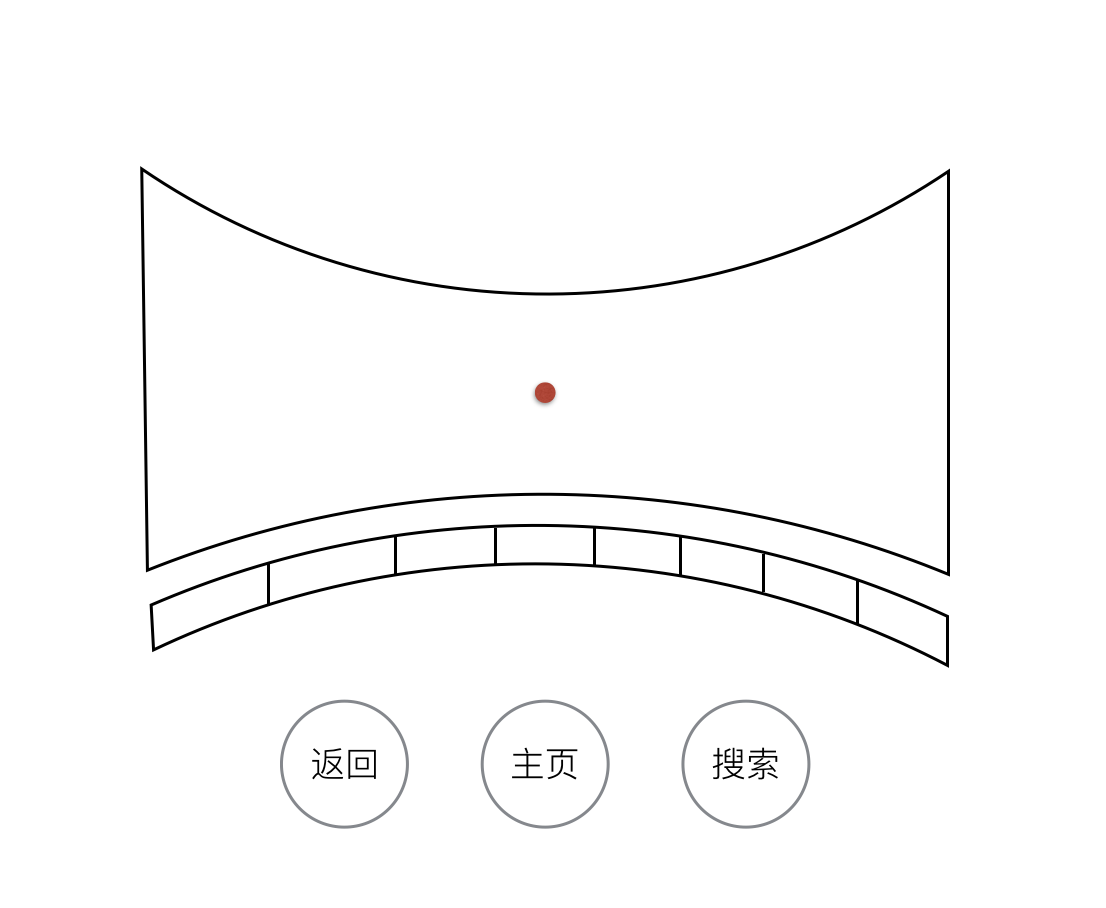
\includegraphics[width=.5\textwidth]{menu}
}
\caption{类别界面设计}
\label{fig:menu}
\end{figure}

\subsection{漫游界面设计}
\begin{itemize}
	\item 漫游界面带有紧急退出区域,只需注视 1~2 秒以上就可以紧急退出场景,避免眩晕加重。
	\item 可通过地面上的指示图标切换场景。
	\item 可通过场景中的热点区域查看详细信息。
\end{itemize}
如图\ref{fig:scenery}。

\begin{figure}[htp]
\centering
\fbox{
  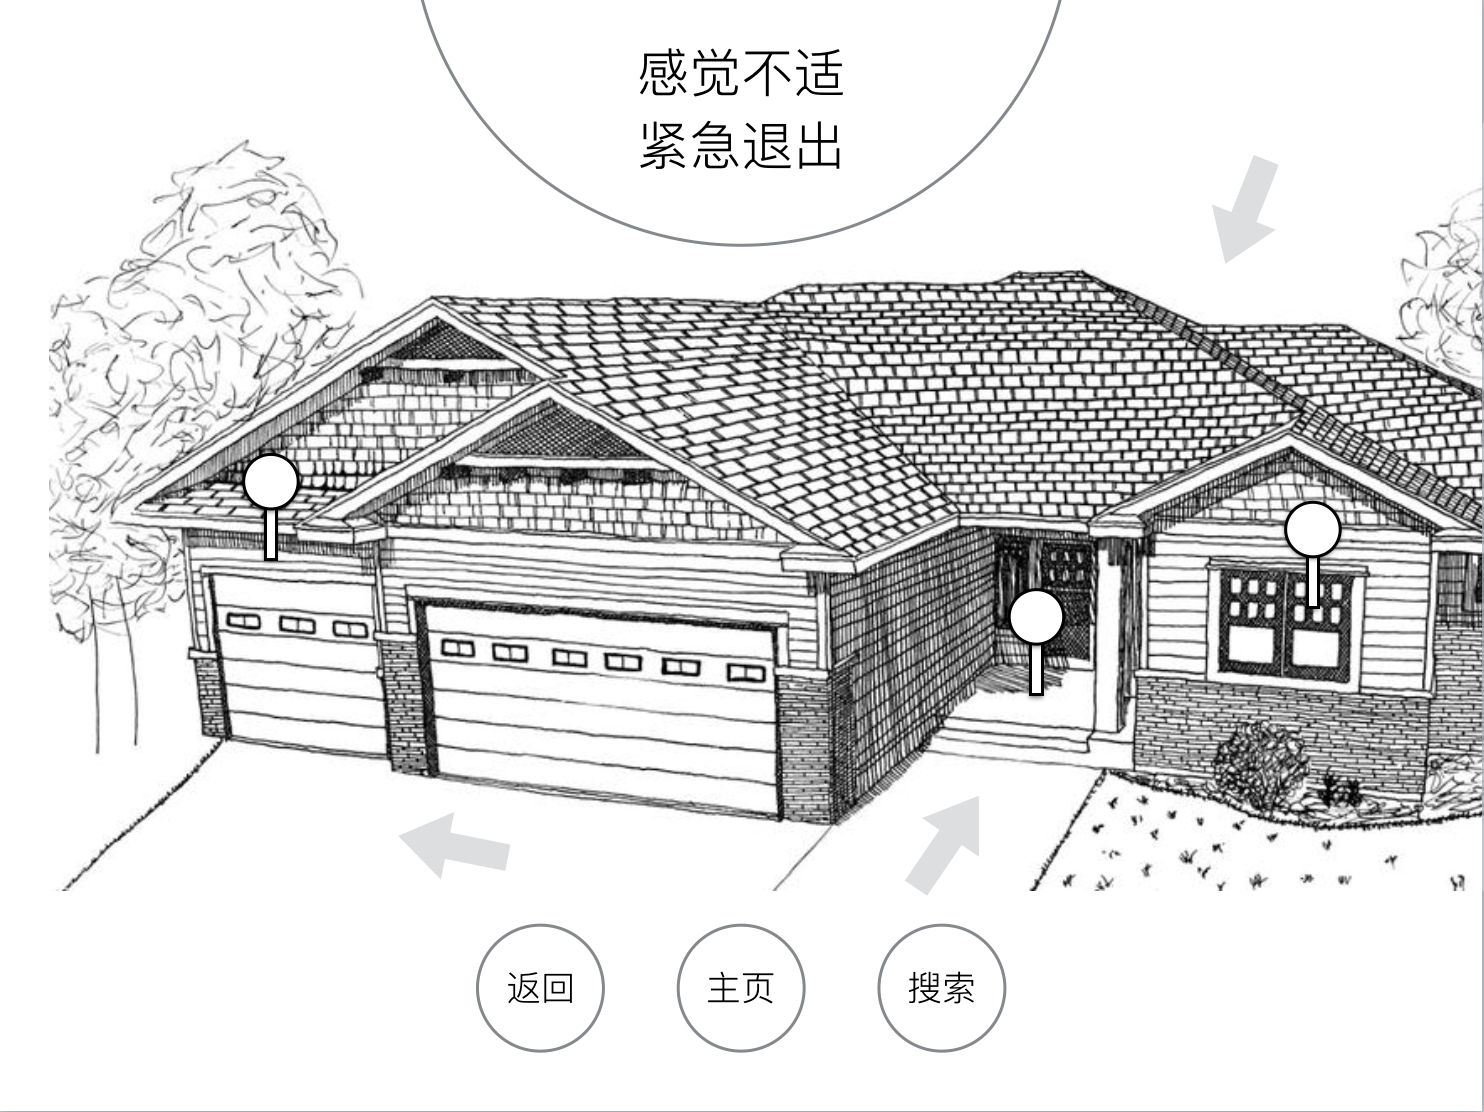
\includegraphics[width=.5\textwidth]{scenery}
}
\caption{漫游界面设计}
\label{fig:scenery}
\end{figure}

\subsection{设置界面设计}
设置界面可通过注视相关范围控件以调节参数,如图\ref{fig:setting}。

\begin{figure}[htp]
\centering
\fbox{
  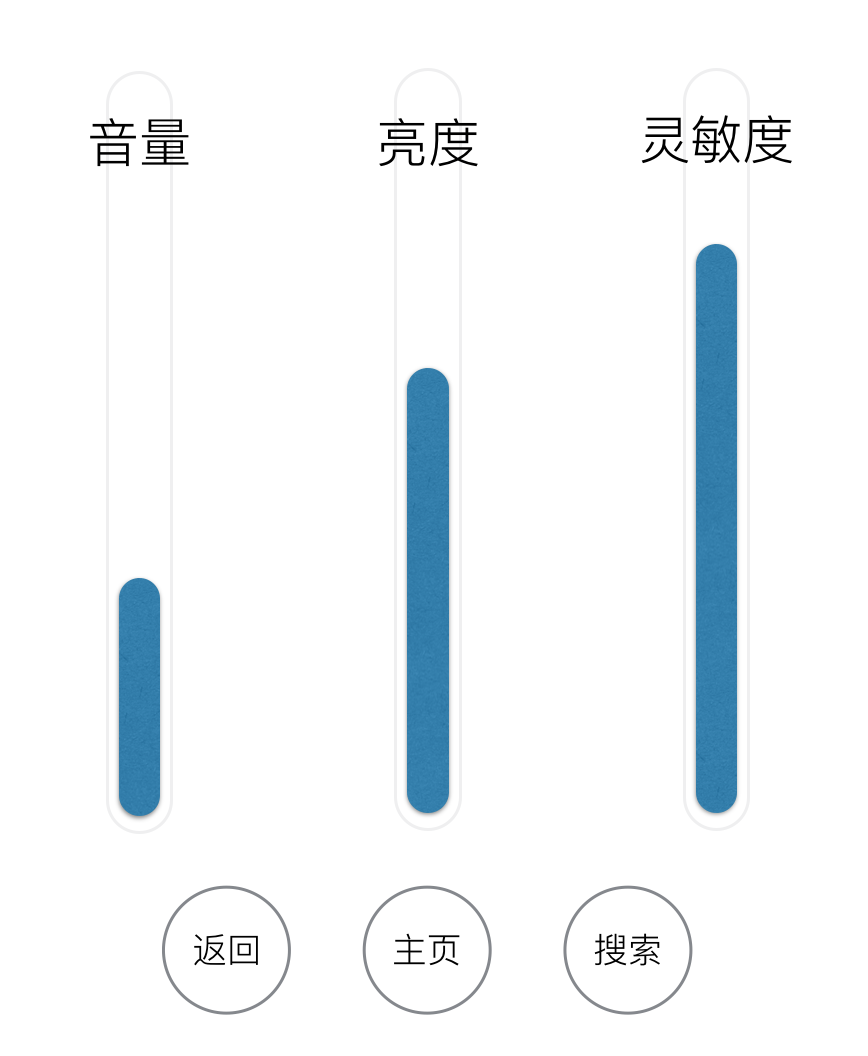
\includegraphics[width=.5\textwidth]{setting}
}
\caption{设置界面设计}
\label{fig:setting}
\end{figure}

\subsection{未完待续}
